\documentclass{xjtureport}
% =============================================
% Part 0 Edit the info
% =============================================

\major{计算机科学与技术}
\name{曾锦程}
\title{软件定义网络实验报告}
\stuid{2203613040}
\college{计算机学院}
\date{\zhtoday}
\lab{Personal Device}
\course{软件定义网络}
\instructor{张鹏}
\grades{}
\expname{The Process of Network}
\exptype{}
\partner{}

\begin{document}
% =============================================
% Part 1 Header
% =============================================
\makecover
\makeheader

% =============================================
% Part 2 Main document
% =============================================

\section{实验目的和要求}
Use Wireshark to understand the process of network communication.\par
–Capture as more protocol packets as possible, including but not limited to DHCP, ARP, DNS, HTTP, TCP, UDP, …\par
–A report that describes the detailed communication process, and what you newly understand after this Wireshark lab
\section{实验内容和步骤}
–Start your device from a clean state, without an IP address\par
–Run Wireshark to capture packets\par
–Use your browser to visit a website (e.g., www.baidu.com)\par
–Read the captured packets in sequence\par
\section{实验环境}
计算机,Wireshark, 个人服务器43.143.132.10以及域名www.zjcblog.top, QQ。
\section{实验过程}
\subsection{将电脑设为clean state}
使用命令:\par
\begin{center}
	\texttt{netsh interface ip set address name="WLAN" static 地址+子网掩码+网关}
\end{center}\par
将原本动态设置IP地址设置为静态(当重新设置成动态后,主机会向DHCP服务器发包,就能达到clean state的效果)。\par
\begin{figure}[H]
	\centering
	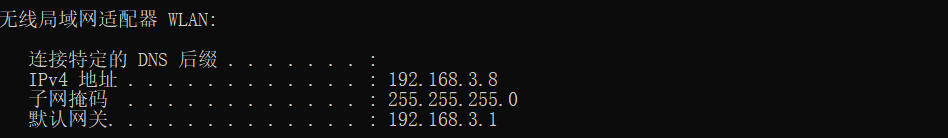
\includegraphics[width=0.8\linewidth]{wlan.png}
	\caption{手动设置IP地址后WLAN}
\end{figure}
\begin{figure}[H]
	\centering
	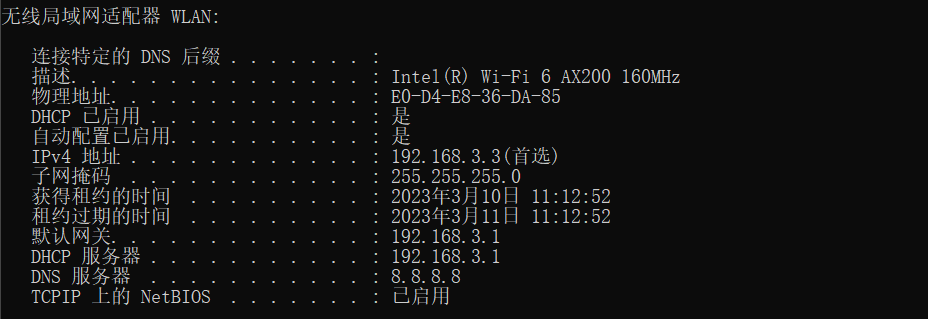
\includegraphics[width=0.8\linewidth]{zidong.png}
	\caption{自动设置IP地址后WLAN}
\end{figure}
使用命令:\par
\begin{center}
	\texttt{ipconfig /flushdns}
\end{center}\par
来刷新dns缓存,把dns服务器设置成8.8.8.8(谷歌dns服务器)。
\begin{figure}[H]
	\centering
	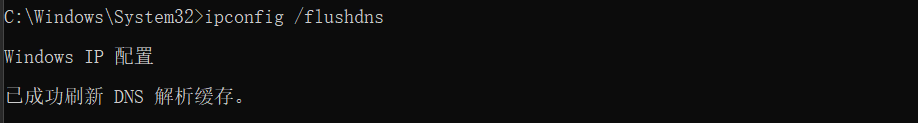
\includegraphics[width=0.8\linewidth]{flushdns.png}
	\caption{刷新DNS缓存}
\end{figure}
\subsection{Wireshark抓包}
保证在设置静态IP地址后开始使用Wireshark来抓包,接口选择WLAN口,之后开始捕获。
\begin{figure}[H]
	\centering
	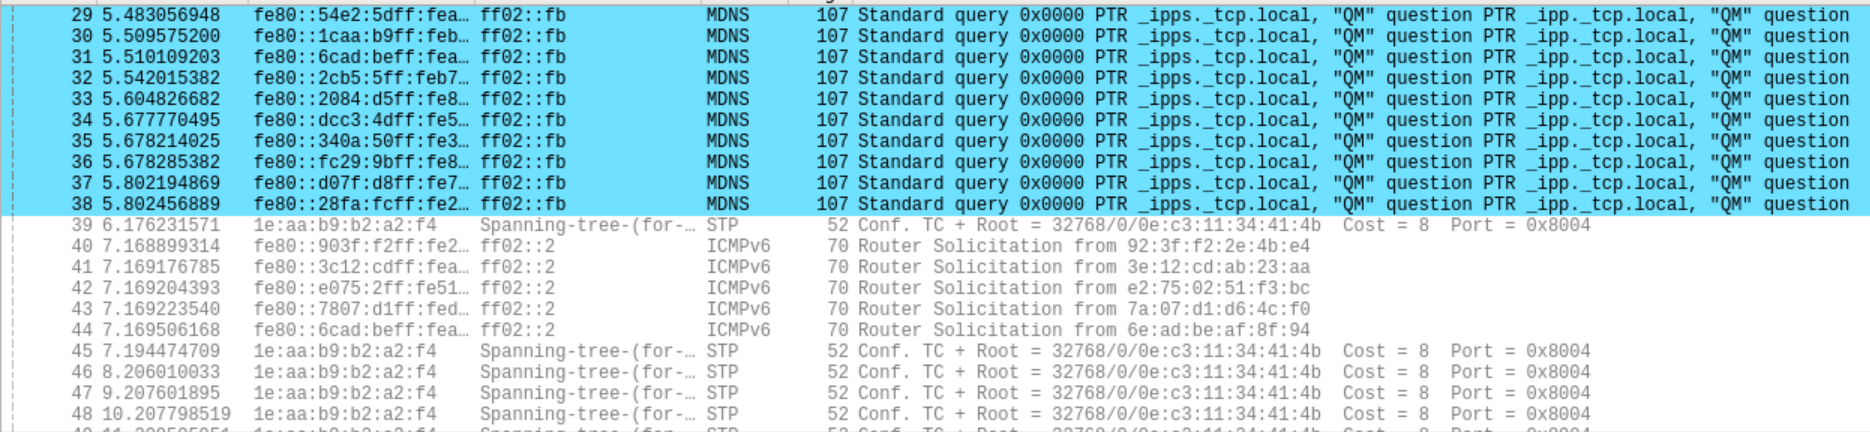
\includegraphics[width=0.8\linewidth]{wireshark.png}
	\caption{wireshark选择接口}
\end{figure}
\subsection{打开网站和应用}
在抓包过程中打开QQ和个人服务器网站www.zjcblog.top以及www.bilibili.com,进行实验观察,并进行协议分析。
\begin{figure}[H]
	\centering
	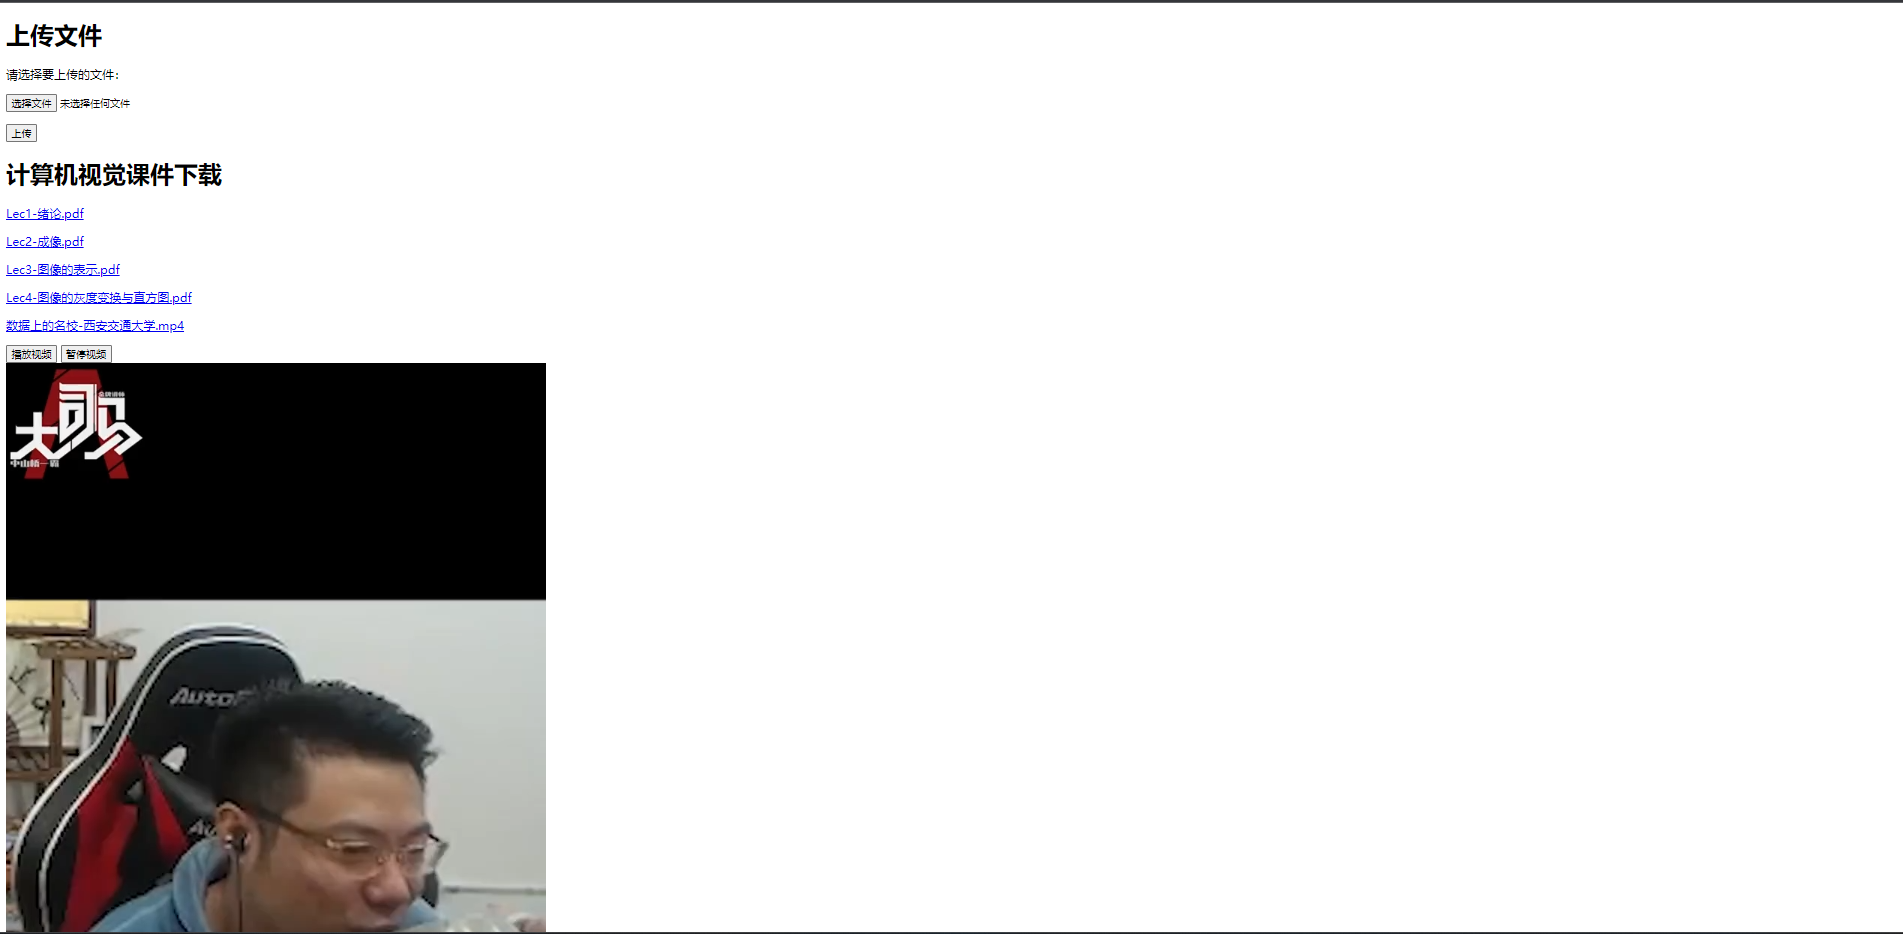
\includegraphics[width=0.8\linewidth]{wangzhan.png}
	\caption{www.zjcblog.top上提供的上传、下载、播放视频接口}
\end{figure}
\section{上网协议分析}
\subsection{DHCP}
开启filter:dhcp,发现抓到的包分为四种类型。
\begin{figure}[H]
	\centering
	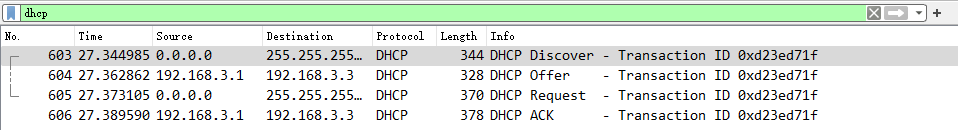
\includegraphics[width=0.8\linewidth]{dhcp.png}
	\caption{抓到的DHCP协议包}
\end{figure}
查阅并分析得知DHCP的基本工作过程如下:\par
(1)寻找DHCP服务器。DHCP客户端(需要动态获得IP地址的主机)启动时,会广播发送一个DHCP发现(DHCP Discover)报文,由于客户端还不知道自己属于哪一个网络,所以IP分组的源地址为0.0.0.0,而目的地址为255.255.255.255。
\begin{figure}[H]
	\centering
	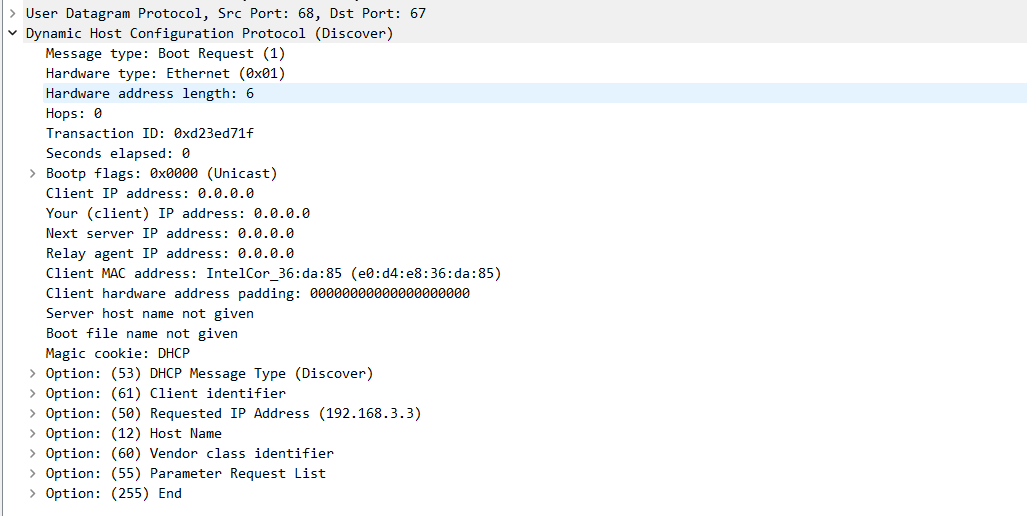
\includegraphics[width=0.8\linewidth]{dhcp-discover.png}
	\caption{DHCP-Discover}
\end{figure}
(2)提供IP租用地址。当DHCP服务器监听到客户端广播发送的DHCP发现报文后,它会从那些还没有租出的地址范围内选择最前面的空置IP地址,连同其他TCP/IP协议设定,应答给DHCP客户端一个DHCP提供(DHCP Offer)报文。由于客户端在开始的时候还没有IP地址,所以在其提供报文中会带有请求DHCP客户端的MAC地址信息。根据服务器端的设定,提供报文中还会包含一个租约期限的信息。
\begin{figure}[H]
	\centering
	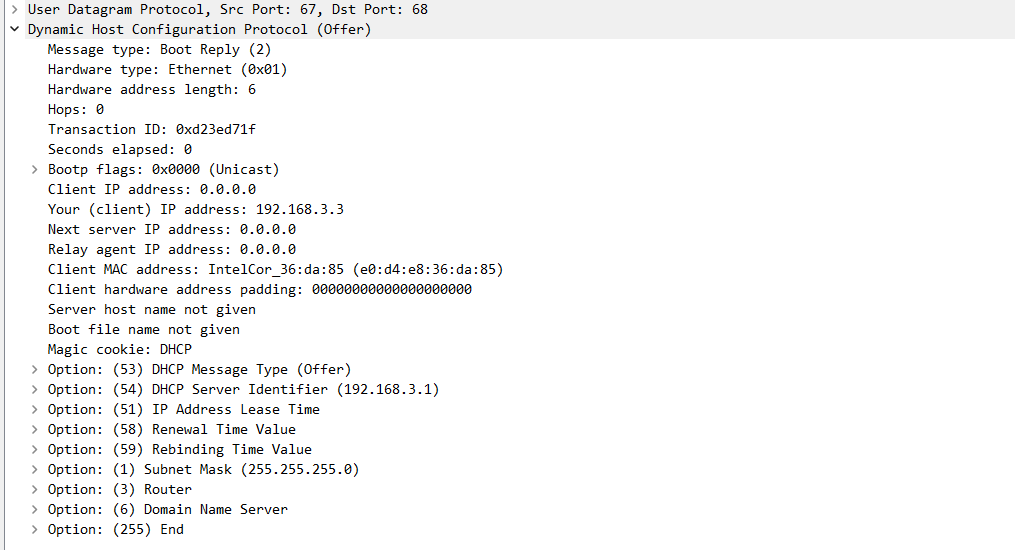
\includegraphics[width=0.8\linewidth]{dhcp-offer.png}
	\caption{DHCP-Offer}
\end{figure}
(3)接收IP租约。如果DHCP客户端受到网络多台DHCP服务器的提供报文,只会挑选并接受其中的一个提供报文(通常是最先抵达的那个),并且会广播发送一个DHCP请求报文,报文中包含选中的DHCP服务器的IP地址和需要的IP地址。\par 
同时,客户端还会向网络发送一个ARP报文,查询网络上是否有其他机器使用该IP地址;如果发现该IP地址已经被占用,客户端则会发送一个DHCP Decline报文给DHCP服务器,拒绝接收其DHCP提供报文,并重新广播发送DHCP发现报文。(这里DHCP提供的IP地址并不发生冲突,所以没有出现该种包)
\begin{figure}[H]
	\centering
	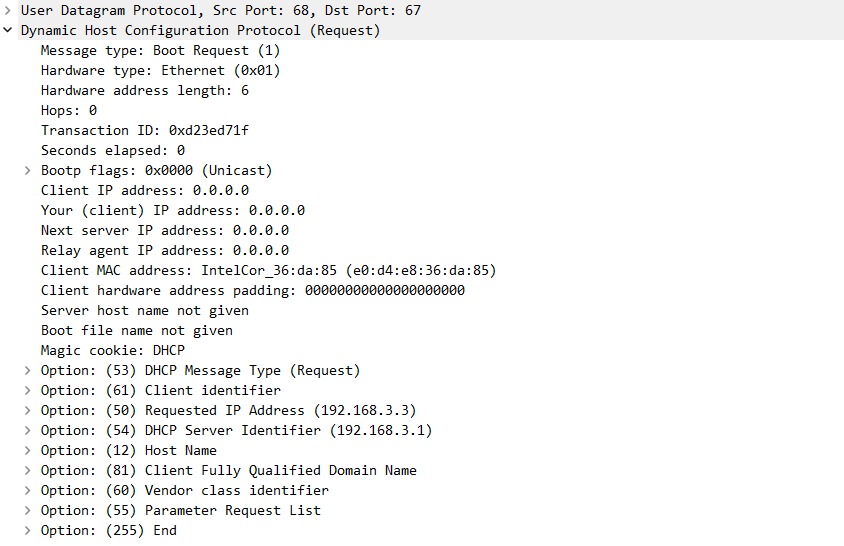
\includegraphics[width=0.7\linewidth]{dhcp-request.png}
	\caption{DHCP-Request}
\end{figure}
(4)租约确认。当DHCP服务器接收到客户端的DHCP请求报文后,判断报文中IP地址是否与自己的地址相同。如果不相同,则DHCP服务器不做任何处理,只清除相应IP地址分配记录;如果相同,DHCP服务器就会向DHCP客户端响应一个DHCP ACK报文,并在选项字段中增加IP地址的使用租期信息,以确认IP的租约正式生效,也就结束了一个完整的DHCP工作过程。
\begin{figure}[H]
	\centering
	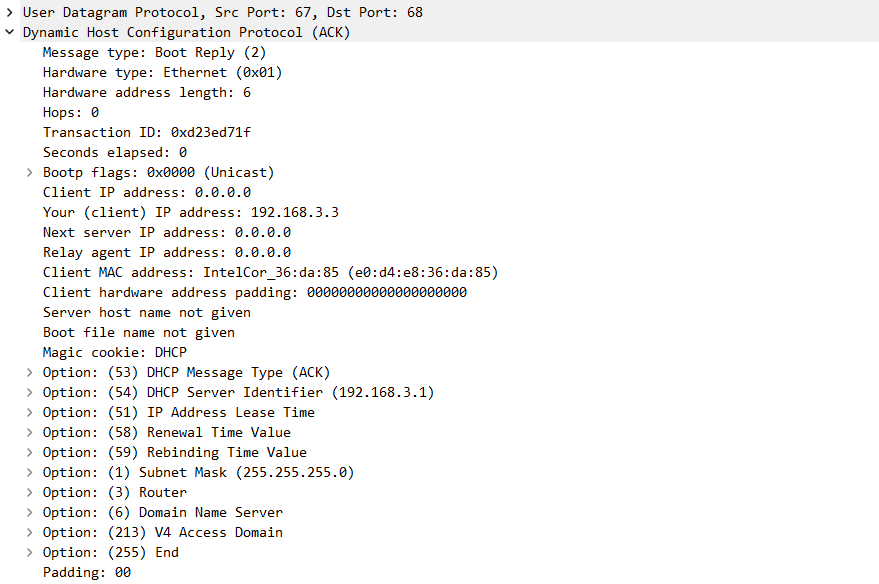
\includegraphics[width=0.8\linewidth]{dhcp-ack.png}
	\caption{DHCP-ACK}
\end{figure}
完整的工作图示如下图所示:
\begin{figure}[H]
	\centering
	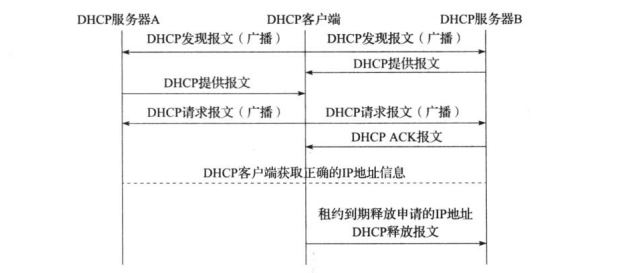
\includegraphics[width=0.8\linewidth]{dhcpgzgc.png}
	\caption{DHCP的基本工作工程}
\end{figure}
\subsection{ARP}
开启filter:arp,发现抓到的包分为两种类型。
\begin{figure}[H]
	\centering
	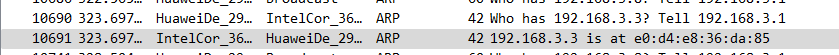
\includegraphics[width=0.8\linewidth]{arp.png}
	\caption{抓到的ARP包}
\end{figure}
(1)发送ARP请求广播:设备会发送一个广播的ARP请求,请求目标设备的MAC地址。这个请求包含了目标设备的IP地址。
\begin{figure}[H]
	\centering
	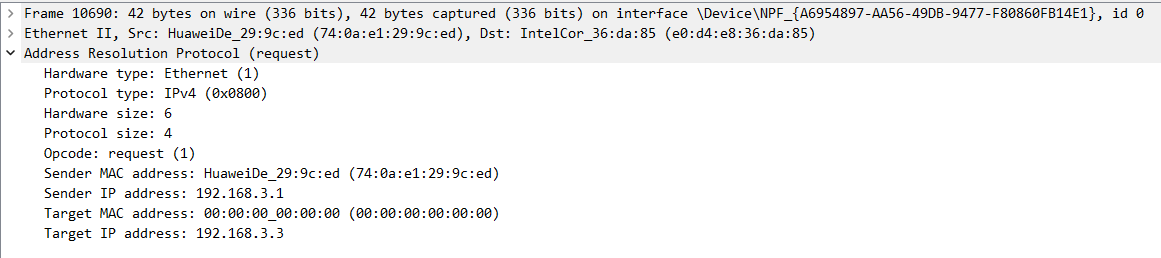
\includegraphics[width=0.8\linewidth]{arp-request.png}
	\caption{ARP-Request}
\end{figure}
(2)ARP响应包被发送回到源设备:源设备接收到ARP响应包后,将目标设备的MAC地址存储到其ARP缓存中。
\begin{figure}[H]
	\centering
	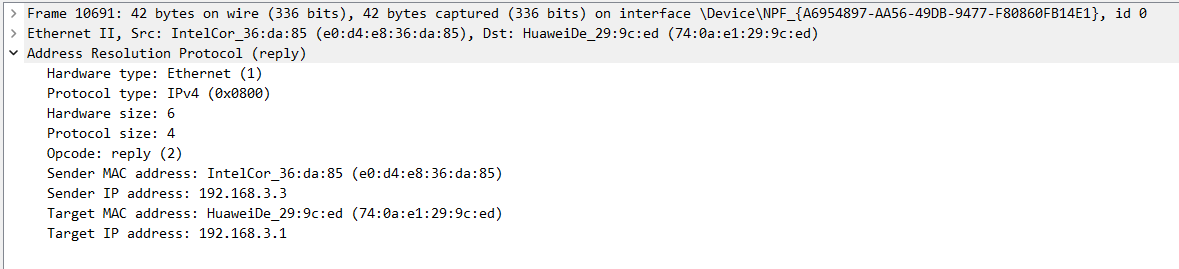
\includegraphics[width=0.8\linewidth]{arp-reply.png}
	\caption{ARP-Reply}
\end{figure}

\subsection{DNS}
从浏览器输入www.zjcblog.top,并开启filter:arp,发现抓到三个包。
\begin{figure}[H]
	\centering
	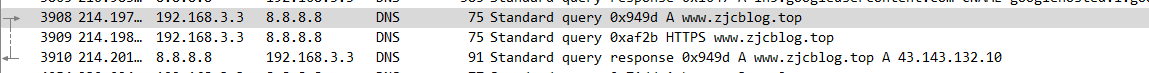
\includegraphics[width=0.8\linewidth]{dns.png}
	\caption{抓到的DNS包}
\end{figure}
(1)DNS-Query-A\par
DNS的A类型报文即建立一个域名到IP地址的映射,这里是在询问DNS服务器关于www.zjcblog.top的A映射。
\begin{figure}[H]
	\centering
	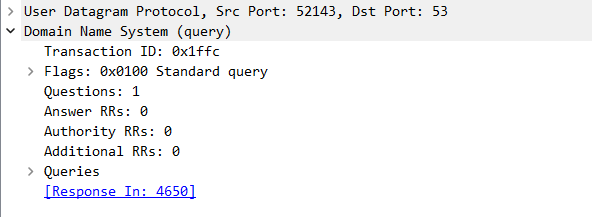
\includegraphics[width=0.8\linewidth]{dns-query.png}
	\caption{DNS-Query-A}
\end{figure}
(2)DNS-Query-HTTPS\par
DNS的HTTPS报文,即在询问该网站是否有HTTPS服务,如果有则导向HTTPS服务器连接。(个人服务器并没有开启HTTPS服务)
\begin{figure}[H]
	\centering
	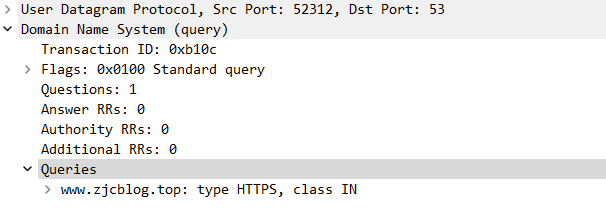
\includegraphics[width=0.8\linewidth]{dns-query-https.png}
	\caption{DNS-Query-HTTPS}
\end{figure}
(2)DNS-Response-A\par
DNS服务器这时候响应主机的请求,返回关于www.zjcblog.top的A映射,然而对于谷歌服务器来说则会同时返回服务器的认证服务器。\par
对于DNS服务器查询来说其实还分为递归查询和迭代查询,递归查询则不会返回目的dns服务器的地址,而迭代则会,同时让主机查询目的DNS服务器,这里则返回了目的DNS服务器。
\begin{figure}[H]
	\centering
	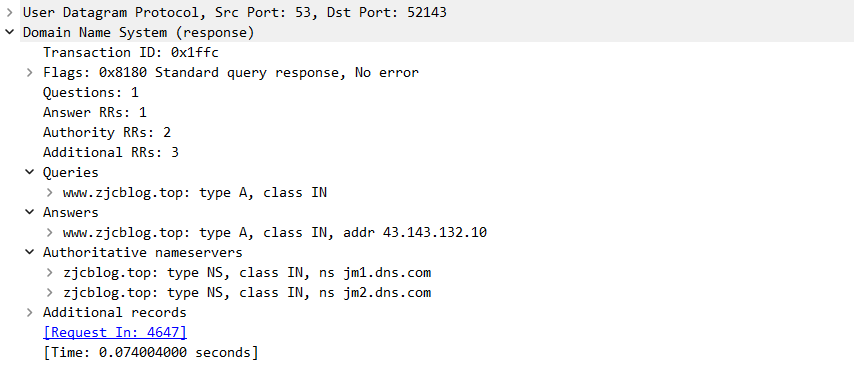
\includegraphics[width=0.8\linewidth]{dns-response.png}
	\caption{DNS-Response-A}
\end{figure}
\subsection{TCP}
同时在www.zjcblog.top中开始使用接口(上传、下载、播放视频)并抓包,并开启filter:ip.addr == 43.143.132.10 and tcp:
\begin{figure}[H]
	\centering
	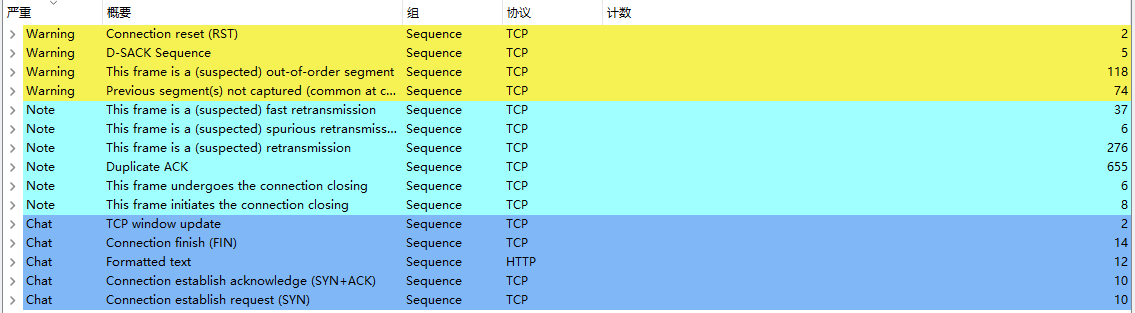
\includegraphics[width=0.8\linewidth]{tcp.png}
	\caption{TCP统计图}
\end{figure}
可以看出其中传送的TCP包非常多,这里只对部分包进行介绍。\par
(1)三次握手过程
\begin{figure}[H]
	\centering
	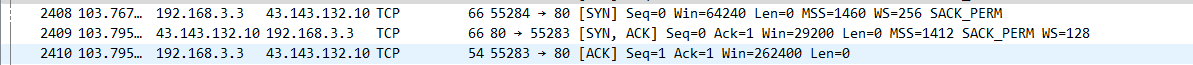
\includegraphics[width=0.8\linewidth]{sanciwoshou.png}
	\caption{三次握手过程}
\end{figure}
(2)挥手过程
\begin{figure}[H]
	\centering
	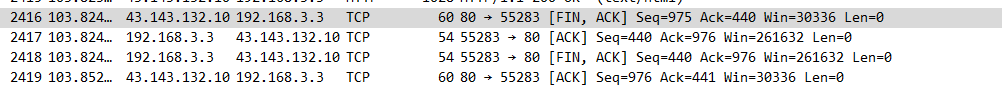
\includegraphics[width=0.8\linewidth]{sicihuishou.png}
	\caption{四次挥手过程}
\end{figure}
\begin{figure}[H]
	\centering
	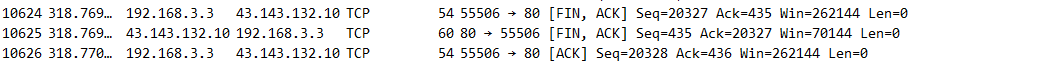
\includegraphics[width=0.8\linewidth]{sancihuishou.png}
	\caption{三次挥手过程}
\end{figure}
(3)流量控制\par 
在下载文件时,发现TCP传送过程中的窗口尺寸变化如下,其中窗口尺寸不断变化,进行流量控制:
\begin{figure}[H]
	\centering
	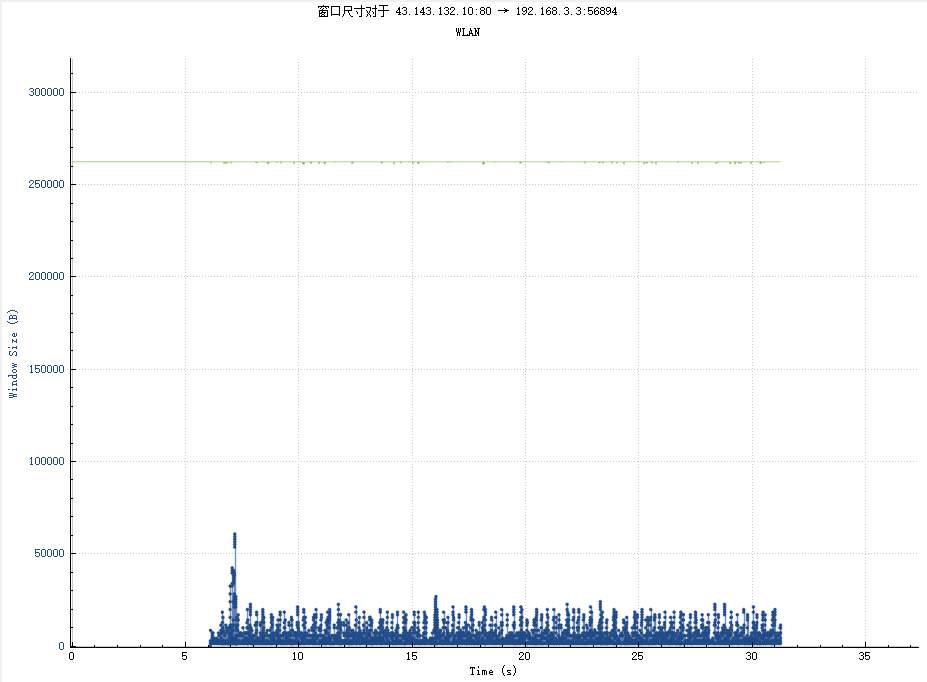
\includegraphics[width=0.8\linewidth]{tcp-download.png}
	\caption{窗口尺寸变化图}
\end{figure}
(4)快速重传\par
使用快速重传进行拥塞控制。
\begin{figure}[H]
	\centering
	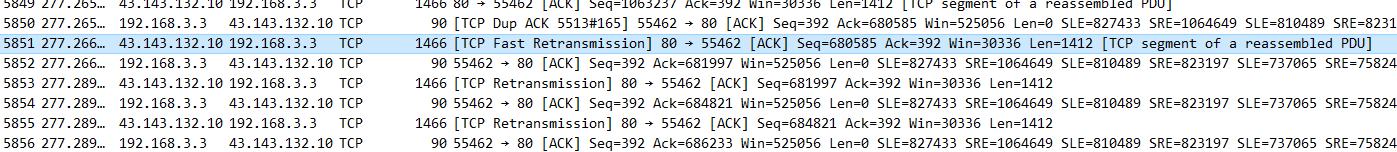
\includegraphics[width=0.8\linewidth]{tcpkuaisuchongchuan.png}
	\caption{快速重传}
\end{figure}
(5)重传\par
\begin{figure}[H]
	\centering
	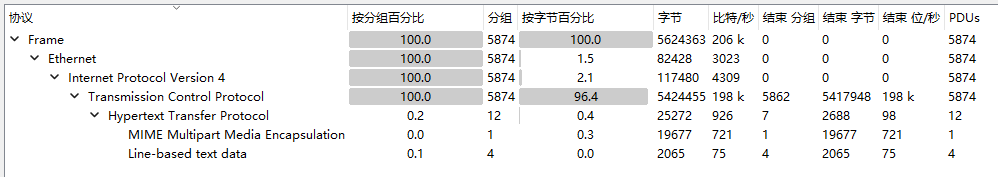
\includegraphics[width=0.8\linewidth]{tcpsum.png}
	\caption{TCP总数}
\end{figure}
\begin{figure}[H]
	\centering
	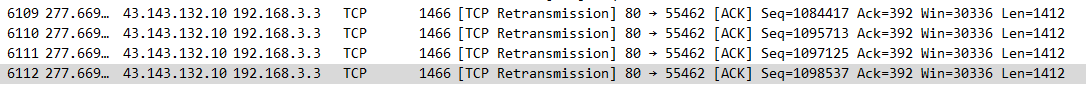
\includegraphics[width=0.8\linewidth]{TCPchongchuan.png}
	\caption{重传}
\end{figure}
可以计算出重传率为4.7\% \par
(6)播放视频\par 
在捕获udp包时播放了网站的mp4视频,发现没有捕捉到udp,而是仍使用的HTTP即TCP,说明TCP也可以偶尔传输视频信息等等。这里也猜测是网页代码编写问题,导致播放视频本质是请求文件导致不是流媒体播放,则不是UDP。
\begin{figure}[H]
	\centering
	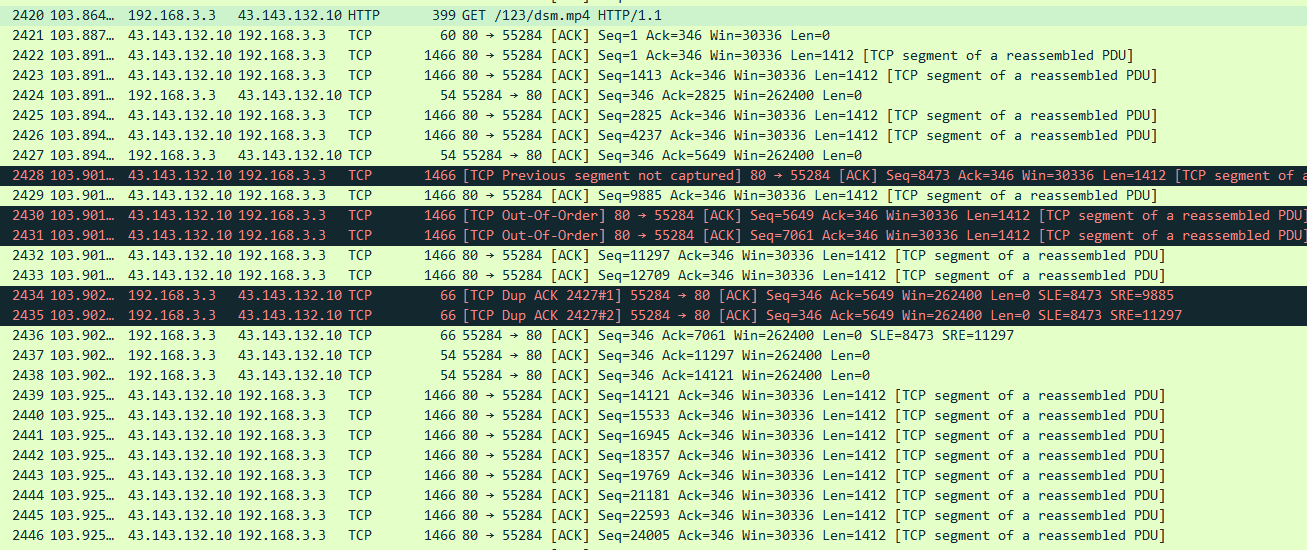
\includegraphics[width=0.8\linewidth]{tcpbofangshiping.png}
	\caption{TCP播放视频}
\end{figure}
\subsection{UDP}
这里通过QQ与宿舍好友开启语音通话,开启UDP传输:
\begin{figure}[H]
	\centering
	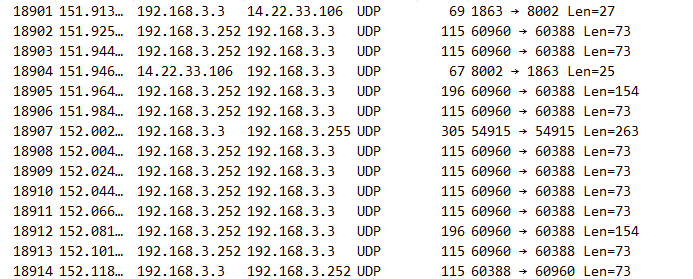
\includegraphics[width=0.8\linewidth]{OICQyuyingchuanshu.png}
	\caption{语音通话中的UDP}
\end{figure}
同时之前的DNS、DHCP其实都是UDP包,主要传输控制信息,且数据长度低,适合无连接的UDP传输。
\subsection{HTTP}
同时在www.zjcblog.top中开始使用接口(上传、下载、播放视频)并抓包,并开启filter:ip.addr == 43.143.132.10 and http:
\begin{figure}[H]
	\centering
	\includegraphics[width=0.8\linewidth]{http.png}
	\caption{抓到的HTTP包}
\end{figure}
(1)主机发出GET,期望与网页进行访问连接。
\begin{figure}[H]
	\centering
	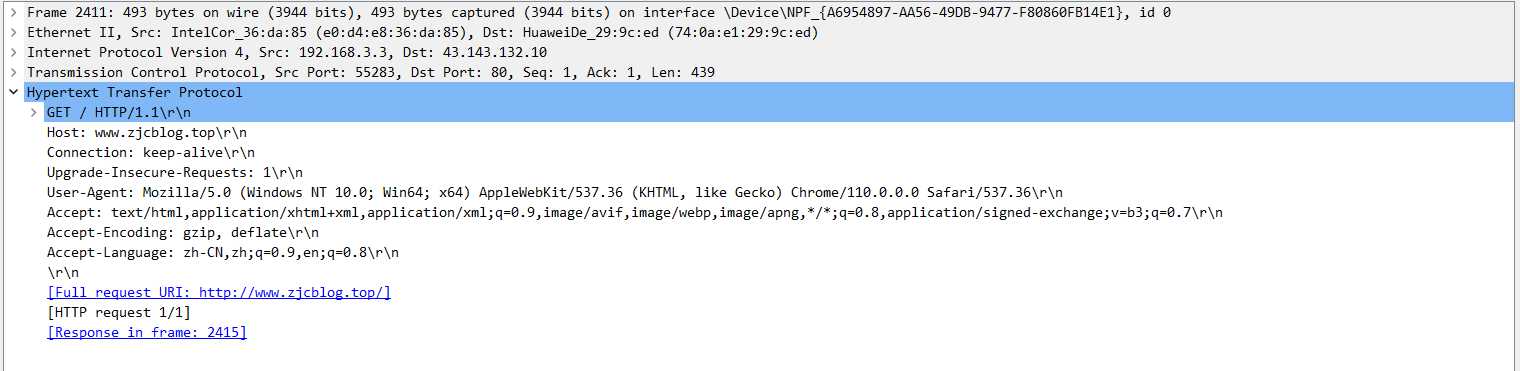
\includegraphics[width=0.8\linewidth]{http-GET.png}
	\caption{HTTP-GET}
\end{figure}
(2)服务器回应,状态码200代表成功访问连接。
\begin{figure}[H]
	\centering
	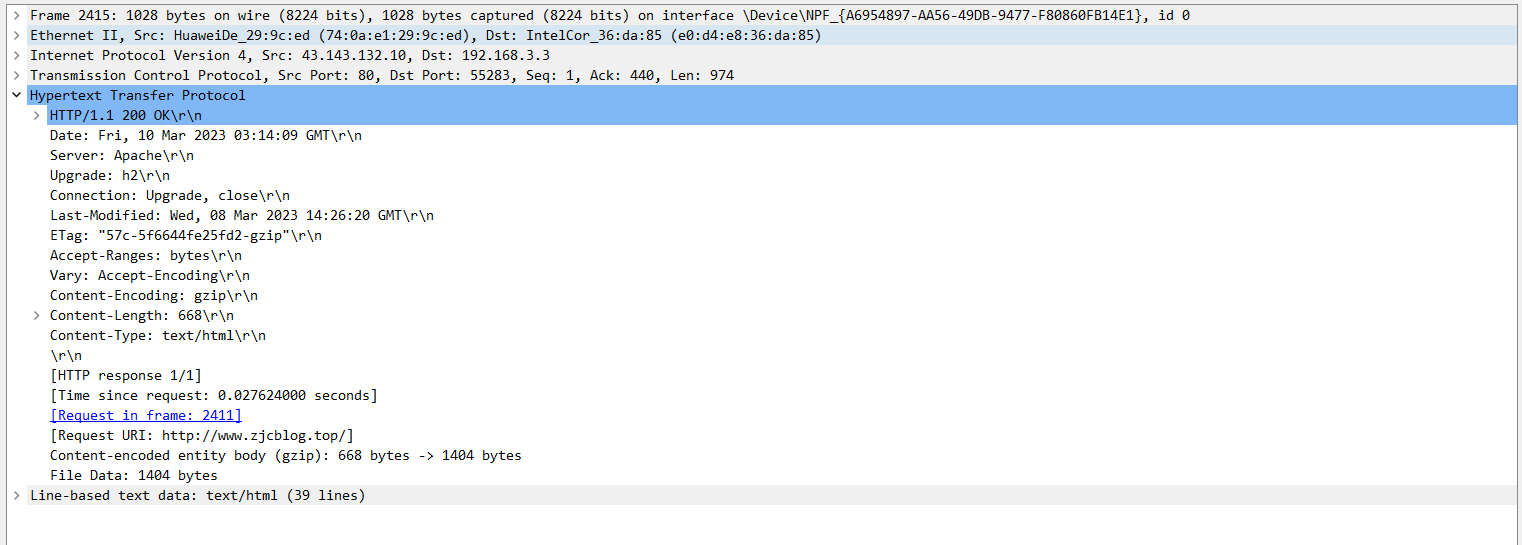
\includegraphics[width=0.8\linewidth]{http-200.png}
	\caption{HTTP-200}
\end{figure}
(3)主机向服务器请求网页文件,需要使用GET,比如如下图的视频文件。
\begin{figure}[H]
	\centering
	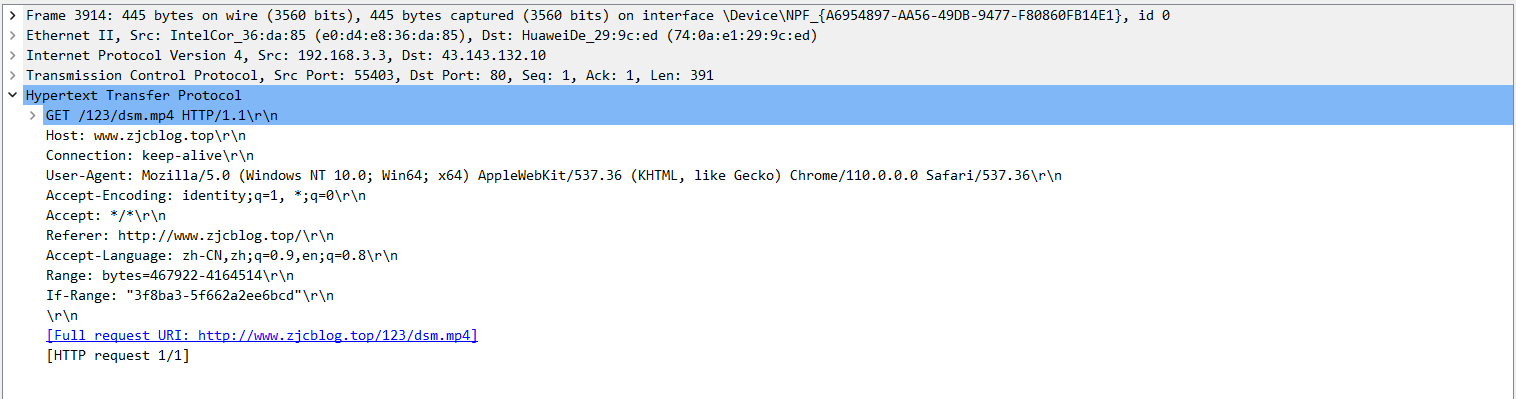
\includegraphics[width=0.8\linewidth]{http-mp4-tcp.png}
	\caption{HTTP-GET}
\end{figure}
(4)主机上传文件时,需要使用POST,这里上传的是一张图片,于是会再封装一层MIME协议,用于HTTP的多媒体传输服务:
\begin{figure}[H]
	\centering
	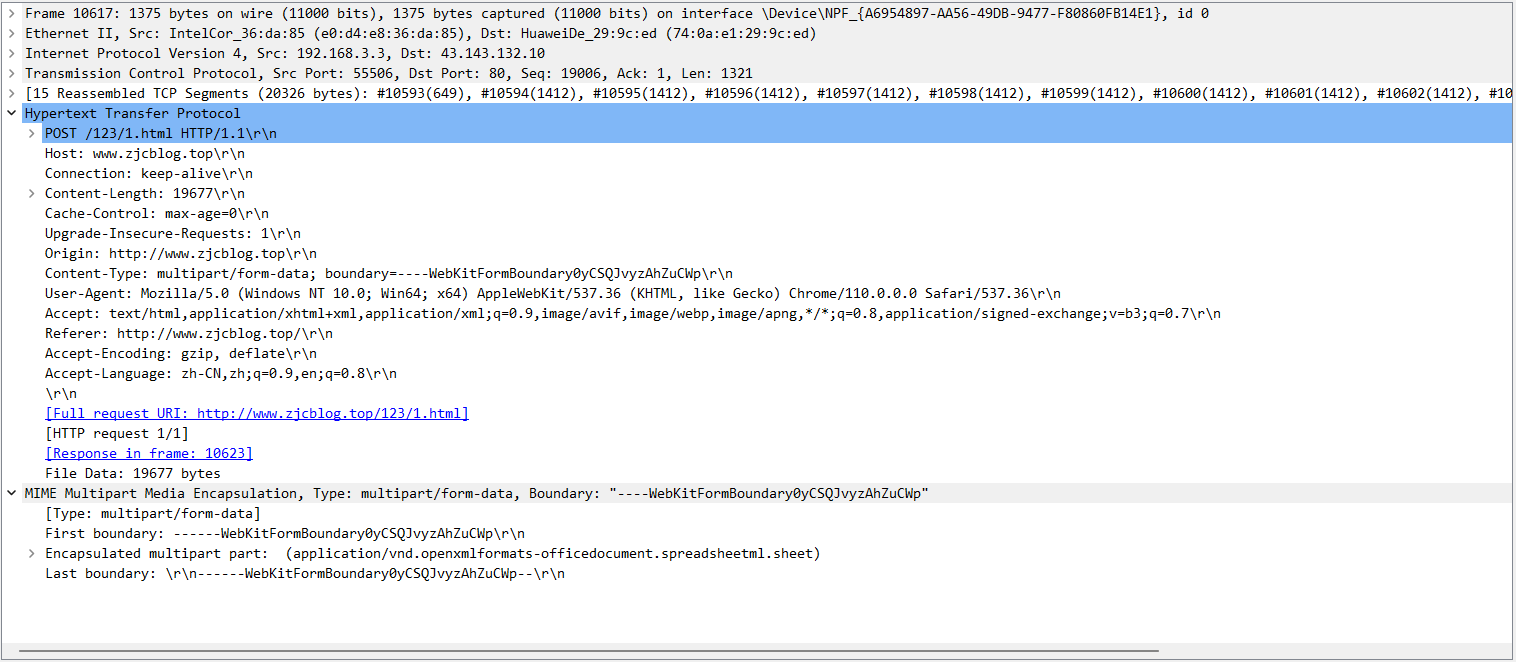
\includegraphics[width=0.8\linewidth]{http-mime-post.png}
	\caption{HTTP-POST}
\end{figure}

\subsection{OICQ}
在登录QQ的时候,发现了OICQ协议,现对其进行抓包分析:\par
以下是刚打开QQ登录时抓到的包,TLSv1.2与SSL都是保证传输层安全的协议,其他数据包则主要用于建立起客户端到QQ服务器的连接,三次握手等等。
\begin{figure}[H]
	\centering
	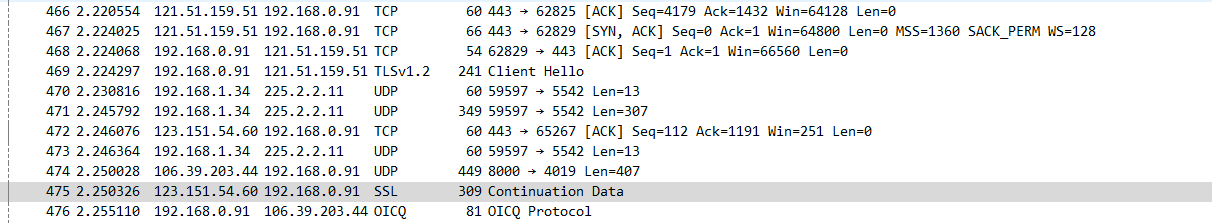
\includegraphics[width=0.8\linewidth]{OICQbefore.png}
	\caption{OICQ-Before}
\end{figure}
(1)登录\par
然而值得注意的是,这实际上是关闭QQ即账号下线抓到的,语义相反。
\begin{figure}[H]
	\centering
	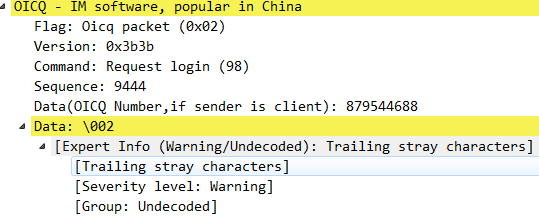
\includegraphics[width=0.8\linewidth]{OICQdengchu.png}
	\caption{OICQ-Login}
\end{figure}
(2)登出\par
然而值得注意的是,这实际上是登录QQ时候抓到的,语义相反。
\begin{figure}[H]
	\centering
	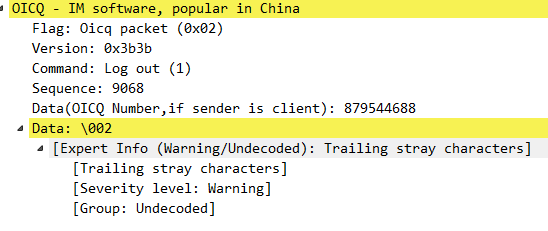
\includegraphics[width=0.8\linewidth]{OICQdenlu.png}
	\caption{OICQ-Log out}
\end{figure}
(3)获得好友状态
\begin{figure}[H]
	\centering
	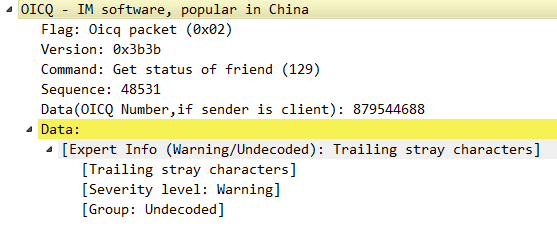
\includegraphics[width=0.8\linewidth]{OICQhuoquhaoyou.png}
	\caption{OICQ-Get status of friend}
\end{figure}
(4)接收消息
\begin{figure}[H]
	\centering
	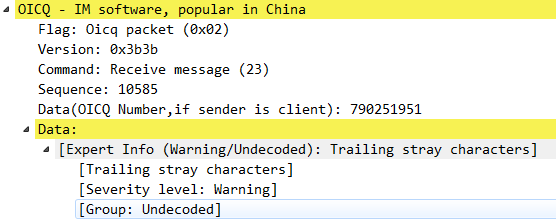
\includegraphics[width=0.8\linewidth]{OICQjieshouxiaoxi.png}
	\caption{OICQ-Receive message}
\end{figure}
(5)设置账号状态
\begin{figure}[H]
	\centering
	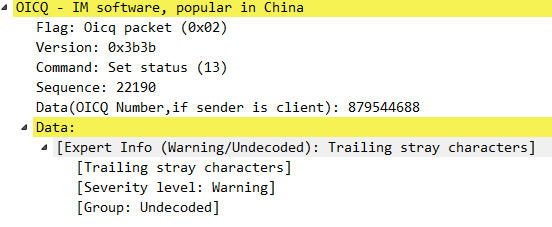
\includegraphics[width=0.8\linewidth]{OICQshezhizhuangtai.png}
	\caption{OICQ-Set status}
\end{figure}
(6)下载朋友列表
\begin{figure}[H]
	\centering
	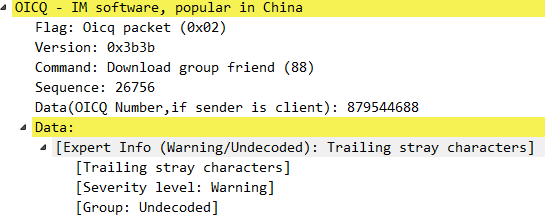
\includegraphics[width=0.8\linewidth]{OICQxiazaihaoyouliebiao.png}
	\caption{OICQ-Download group friend}
\end{figure}
(7)组名操作
\begin{figure}[H]
	\centering
	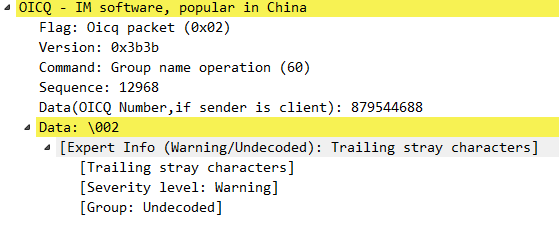
\includegraphics[width=0.8\linewidth]{OICQzumingcaozuo.png}
	\caption{OICQ-Group name operation}
\end{figure}
下图是与舍友QQ语音通话的报文截获图,14.22.33.106为腾讯服务器的IP地址,而在其中发现语音UDP传输从主机到服务器再到主机的模式,更改成了同一局域网中的UDP语音传输,这样大大提高了语音通话质量,是一种很智能的协议模式。
\begin{figure}[H]
	\centering
	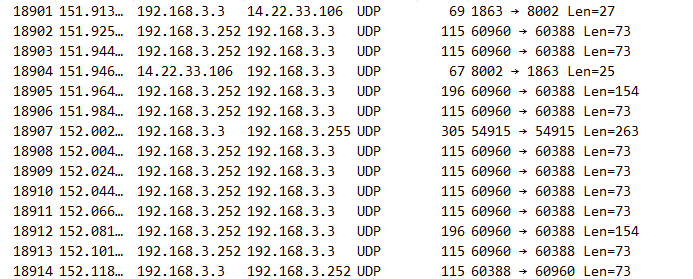
\includegraphics[width=0.8\linewidth]{OICQyuyingchuanshu.png}
	\caption{语音传输链路转移的过程}
\end{figure}
\section{实验感悟}
(1)基本了解了主机上网过程,由上述这些协议共同服务实现,其实除此之外还有NAT协议等等,让我对计算机网络通信又有了更深的理解。\par
(2)发现在网页上播放视频,并不一定就是UDP传输,也有可能是TCP传输,一切都要从实际出发,不能光依赖于理论。\par
(3)学习到了Wireshark抓包软件的各种用法,包括过滤器、专家信息、TCP流图、分级协议统计等等。\par
(4)简单分析了QQ的OICQ协议,发现其报文OICQ - IM software, popular in China很有意思,并且了解了平时对QQ操作的各种协议包。还发现了OICQ的优化链路功能,检测到两台主机为统一局域网下(同一公网IP),从主机到服务器再到主机的UDP语音传输链路,转换成了局域网内主机到主机的UDP语音传输。
\end{document}
